\section{Experiments}

\subsection{Estimator accuracy}

We ran experiments on CIFAR-10 and Imagenet to compare the practical performance of our estimator and the plugin estimator. Suppose we have a model with $B$ outputs that has true $\ell_2^2$ calibration error ${E^*}^2$. Suppose we draw $n$ samples, and obtain estimates $\hat{E}^2$ and $\hat{E}_{pl}^2$ from our estimator and the plugin estimator respectively, where $\hat{E}^2$ and $\hat{E}_{pl}^2$ are random variables. We want to know which of these estimates tends to be closer to the true value ${E^*}^2$. One way is to compare the mean squared error of the estimates: $\mathbb{E}\big[ (\hat{E}^2 - {E^*}^2)^2 \big]$  and $\mathbb{E}\big[ (\hat{E}_{pl}^2 - {E^*}^2)^2 \big]$, for varying values of $B$ and $n$, which we show in Figure~\ref{fig:mse_estimators_bins}. We might also wish to compare histograms of $|\hat{E}^2 - {E^*}^2|$ and $|\hat{E}_{pl}^2 - {E^*}^2|$ for some fixed sample size $n$, which we show in Figure~\ref{fig:histograms_estimators_bins}.

\begin{figure}
  \centering
  \centering
     \begin{subfigure}[b]{0.45\textwidth}
         \centering
         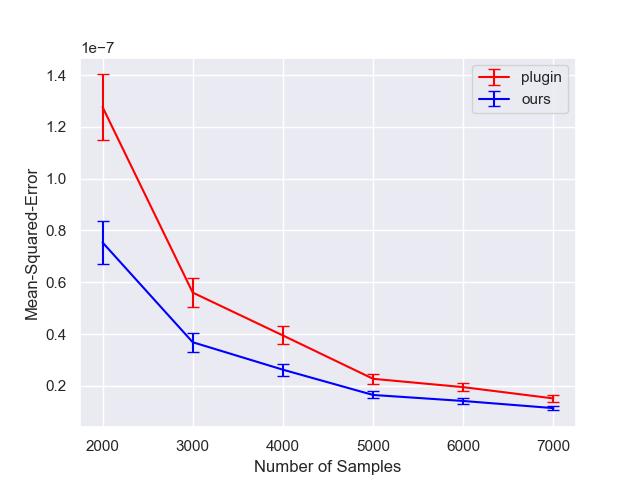
\includegraphics[width=\textwidth]{mse_estimators_10_bins.png}
         \caption{$B$ = 10 bins}
         \label{fig:y equals x}
     \end{subfigure}
     \hfill
     \begin{subfigure}[b]{0.45\textwidth}
         \centering
         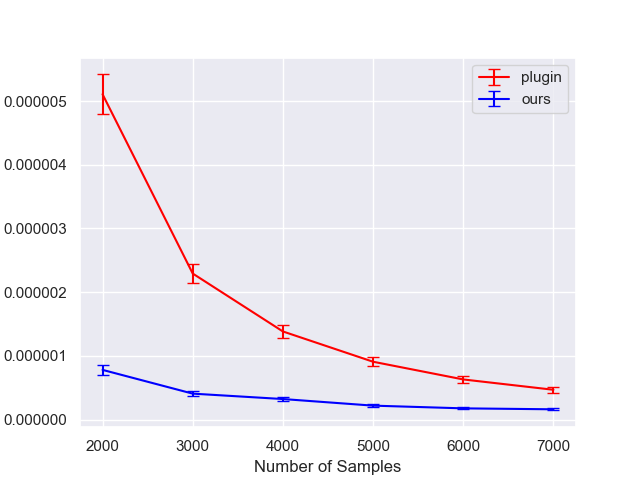
\includegraphics[width=\textwidth]{mse_estimator_100_bins.png}
         \caption{$B = 100$ bins}
         \label{fig:three sin x}
     \end{subfigure}
  \caption{Mean-squared errors of plugin and our estimators on a recalibrated VGG-net model on CIFAR-10 with $90\%$ confidence intervals (lower values better). Our estimator is closer to the ground truth -- the difference between the estimators is more pronounced when the number of bins is higher.}
  \label{fig:mse_estimators_bins}
\end{figure}

\begin{figure}
  \centering
  \centering
     \begin{subfigure}[b]{0.45\textwidth}
         \centering
         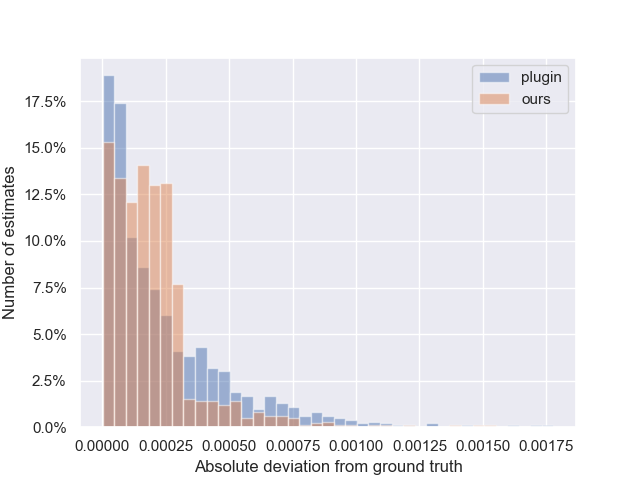
\includegraphics[width=\textwidth]{histogram_estimators_10_bins.png}
         \caption{$B$ = 10 bins}
     \end{subfigure}
     \hfill
     \begin{subfigure}[b]{0.45\textwidth}
         \centering
         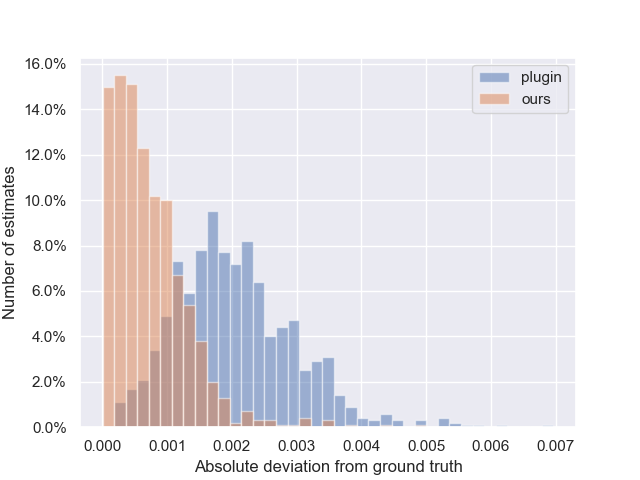
\includegraphics[width=\textwidth]{histogram_estimates_100_bins.png}
         \caption{$B = 100$ bins}
     \end{subfigure}
  \caption{Histograms of the absolute value of the difference between estimated and ground truth $\ell_2^2$ calibration errors. For $B = 10$ bins, the results are mixed but we avoid very bad estimates. For $B=100$ our estimates are much closer to ground truth.}
  \label{fig:histograms_estimators_bins}
\end{figure}


We give an overview of our experimental setup here, with more details in the Appendix, and all code on Github. For CIFAR-10, we used a trained VGG-net model that we recalibrated using Platt scaling on a small held-out set with 1,000 data points. We use 2,000 data points to select $B$ bins to discretize the outputs of the model. The bins were selected so that each bin has an equal number of data points. We use the remaining data points (7,000 for CIFAR-10) for our experiments. 

Suppose we want to evaluate how good our estimates are when they are allowed to use $m$ samples. Ideally, we would draw $m$ samples from the true data distribution, and measure the difference between our estimate and the ground truth. This gives us a single data point, so we would need to do this $T$ times and compute the mean and confidence intervals. This requires an exhaustive amount of data, for example if $m = 5000$ and $T = 100$, we would need 500K data points just for evaluation.

Instead, we approximate the true data distribution with the empirical distribution on the 7,000 data points we have. Then, we measure all quantities with respect to the empirical distribution on the 7,000 data points. That is, we draw samples of size $m$ (with replacement) from the 7,000 data points and run the estimators on these samples. We compare these estimates with the ground truth, the calibration error measured on the empirical distribution. We repeat this $T$ times to get the mean and confidence intervals. This can be viewed as a middle ground between using simulated data, and the impractical ideal where we need 500K CIFAR-10 samples.


\subsection{Model Selection}

Often, the goal is to maximize the predictive quality of the model (for example, as measured by the Brier score), while ensuring that the calibration error is under some threshold $\epsilon$. In our experiment on CIFAR-10, we find that our estimator allows us to select models with a better Brier score subject to a given calibration constraint. The reason for this is that our estimator better bounds the calibration error, which allows us to use more bins while still bounding the calibration error below the desired range (Figure~\ref{fig:mse_vs_ce}. 


We used a trained VGG-net model that we recalibrated using Platt scaling on a small held-out set with 1,000 data points. We use 2,000 data points to select $B$ bins to discretize the outputs of the model, where $B$ ranged from 10 to 100. The bins were selected so that each bin has an equal number of data points. We use the remaining data points (7000 in the case of CIFAR-10) to measure the calibration error. We use bootstrap to estimate the standard error of the estimate, and we report a 95\% upper confidence bound on the estimate. This represents our estimated upper bound on the calibration error. We also report the Brier score. We compute these values for $B = 10, 15, \cdots, 100$ and show the Pareto curve. \footnote{That is, if a point both has worse calibration error and Brier score than another point, we exclude it.} For a given upper bound on the calibration error, our estimator enables us to use more bins which leads to a lower Brier score.
\begin{figure}
  \centering
  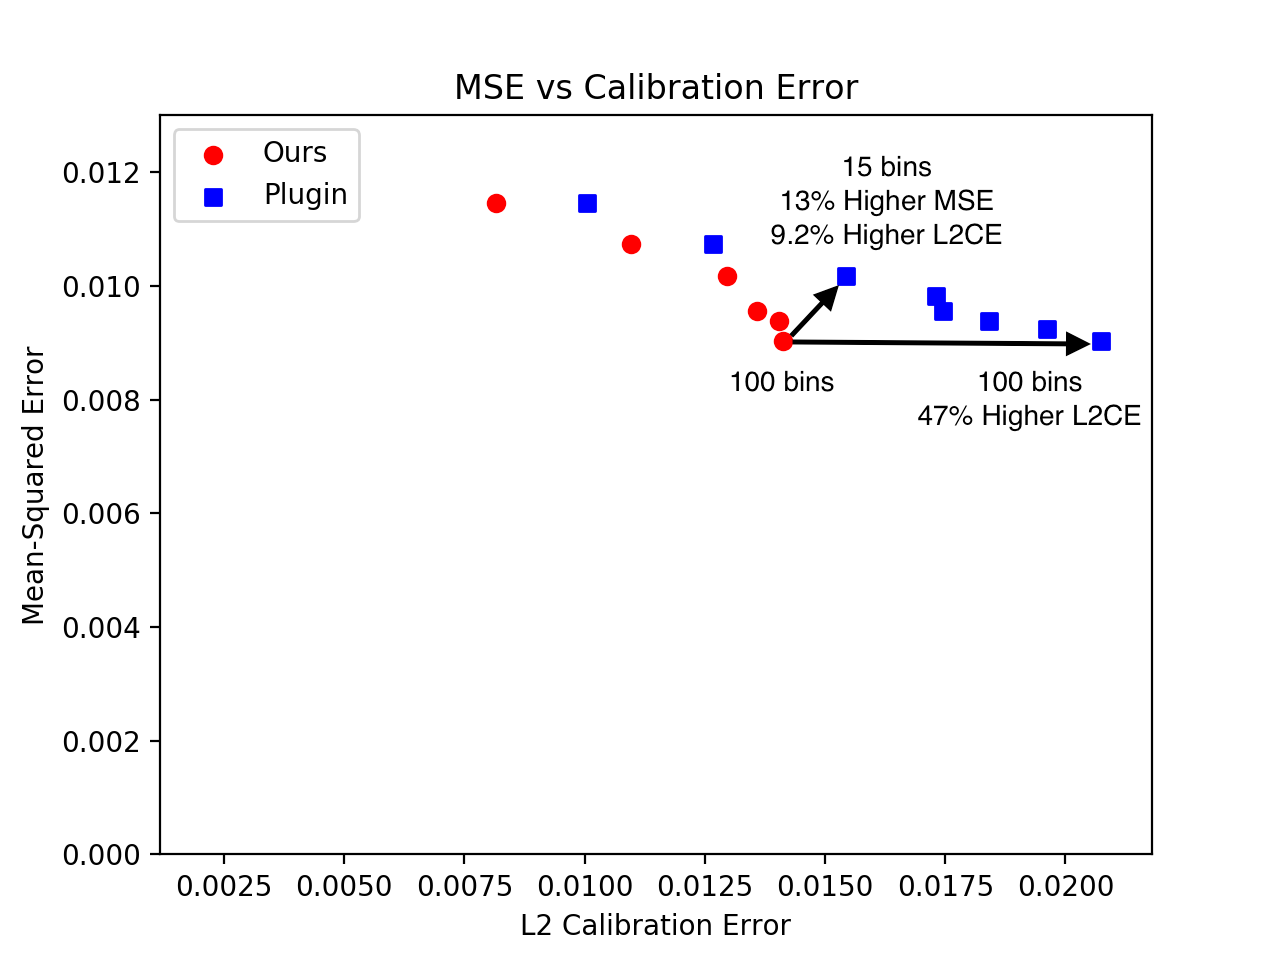
\includegraphics[scale=0.75]{mse_vs_verified_error_plugin_vs_ours.png}
  \caption{Brier scores and upper bounds on the calibration error computed by our estimator and the plugin estimator, when we vary the number of bins $B$. For a given calibration error, our estimator enables us to choose models with a better Brier score. For example, if we want a model with $\ell_2$ calibration error less than 0.015, we can use 100 bins, while the plugin estimator only lets us use 15 bins and incurs a 13\% higher Brier score.}
  \label{fig:mse_vs_ce}
\end{figure}